\documentclass{article}

\usepackage[english]{babel}

\usepackage[letterpaper,top=2cm,bottom=2cm,left=3cm,right=3cm,marginparwidth=1.75cm]{geometry}

% Useful packages
\usepackage{amsmath}
\usepackage{graphicx}
\usepackage[colorlinks=true, allcolors=blue]{hyperref}
\usepackage{listings}
\usepackage[T1]{fontenc}
\usepackage{tgbonum}
\usepackage{textcomp}
\usepackage{setspace}
\usepackage{subcaption}

\usepackage[T1]{fontenc}

\usepackage{xcolor}

\colorlet{punct}{red!60!black}
\definecolor{background}{HTML}{EEEEEE}
\definecolor{delim}{RGB}{20,105,176}
\colorlet{numb}{magenta!60!black}

\lstdefinelanguage{json}{
    basicstyle=\footnotesize\ttfamily,
    stepnumber=1,
    numbersep=8pt,
    showstringspaces=false,
    breaklines=true,
    backgroundcolor=\color{background},
    literate=
     *{0}{{{\color{numb}0}}}{1}
      {1}{{{\color{numb}1}}}{1}
      {2}{{{\color{numb}2}}}{1}
      {3}{{{\color{numb}3}}}{1}
      {4}{{{\color{numb}4}}}{1}
      {5}{{{\color{numb}5}}}{1}
      {6}{{{\color{numb}6}}}{1}
      {7}{{{\color{numb}7}}}{1}
      {8}{{{\color{numb}8}}}{1}
      {9}{{{\color{numb}9}}}{1}
      {:}{{{\color{punct}{:}}}}{1}
      {,}{{{\color{punct}{,}}}}{1}
      {\{}{{{\color{delim}{\{}}}}{1}
      {\}}{{{\color{delim}{\}}}}}{1}
      {[}{{{\color{delim}{[}}}}{1}
      {]}{{{\color{delim}{]}}}}{1}
      {*}{*}{1},
}

\lstdefinestyle{bashStyle}{
  showstringspaces=false,
  language=C,
  basicstyle=\small\sffamily,
  frame=tb,
  columns=fullflexible,
  linewidth=\linewidth,
  xleftmargin=0.075\linewidth,
  breaklines=true,
  literate =
    {'}{{\textquotesingle}}1
    {"}{{\textquotestraightdblbase}}1
    {-}{{-}}1
    {*}{\normalfont{*}}1
}

\title{Modul 1 - Deploying Simple Chat Application using Serverless Technologies}
\author{}

\begin{document}
\lstset{language=C,upquote=true}
\begin{minipage}{0.2\textwidth}
  
\includegraphics[width=\linewidth]{assets/logo_lks.png}
\end{minipage}
\hfill%
\begin{minipage}{0.75\textwidth}
  {\fontfamily{cmr}\selectfont
    {\huge
    \textbf{LOMBA KOMPETENSI SISWA (LKS)}
    \vspace{2mm} 
    \textbf{SEKOLAH MENENGAH KEJURUAN}
    \textbf{TINGKAT KOTA BEKASI}
    \textbf{- 2025}
    }
  }
\end{minipage}
\vspace{30mm} %5mm vertical space
\begin{center}
  {\fontfamily{cmr}\selectfont
    {\huge
      \textbf{NASKAH SOAL}\\
      \vspace{10mm} 
      \textbf{Bidang Lomba}\\
      \vspace{4mm} 
      \textbf{Cloud Computing}
    }
  }
\end{center}
{\let\newpage\relax\maketitle}
\newpage

\begin{figure*}[h]
\centering
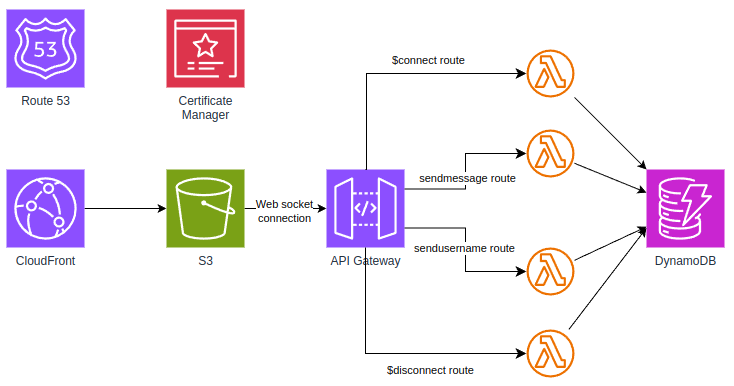
\includegraphics[width=\textwidth]{assets/architecture.png}
\caption{\label{fig:architecture}Architecture Diagram}
\end{figure*}

\section{Overview}
Implementing a serverless architecture on Amazon Web Services (AWS) can provide numerous benefits, including cost optimization, scalability, and reduced administrative burden. Your task is to deploy a simple chat application using serverless architecture.

\section{General Rules}
\begin{enumerate}
    \item Failure to comply with the rules will result in immediate disqualification.
    \item You have 3 hours to finish the tasks.
    \item You may not open any website unless otherwise specified in section \ref{references} and you may open the control panel of your domain provider to update the nameserver to Route 53.
    \item Using the search feature from the AWS documentation website is allowed. However opening other AWS website such as AWS Solutions Library is NOT permitted. If you are unsure about the eligibility of the site you want to open, please ask.
    \item You may use AWS Console, CLI, SAM, CloudFormation, or CDK to deploy the application.
    \item During the event, multiple login is not permitted.
    \item If you have any question, do not hesitate to ask.
\end{enumerate}

\section{Architecture}\label{architecture}

Refer to Figure \ref{fig:architecture}.
\begin{enumerate}
    \item Lambda to handle chat application server's logic.
    \item API Gateway (Websocket APIs) to publish the Lambda via websocket protocol.
    \item DynamoDB to store user information and chat logs.
    \item S3 to host the front-end application.
\end{enumerate}

\section{Information}\label{information}

\begin{enumerate}
  \item The repository URL for the required source code to deploy this solution is:\\
  \href{https://github.com/kensasongko/lksbk2025}{https://github.com/kensasongko/lksbk2025}
  \item This solution must be deployed in \textbf{us-east-1 (North Virginia)} region. Deploying in another region will result in a major point reduction.
  \item An automated scoring system will check your AWS account to calculate the score of your task.
  \item In order check your progress, the scoring system needs an AWS credential with administrator privilege. You will be asked to provide the AWS credential.
  \item AWS tag is used by the scoring system to find your solution. Failing to add the required tag or adding the same tag value to multiple instance may result in an unexpected behavior and thus lower your score.
  \item The system will calculate 90\% of the final score. The remaining 10\% will be evaluated by checking the assignment manually.
  \item If multiple participants completed the assignment, their completion times will factor into the manual scoring process. For instance, the first participant to finish will receive a full score, while subsequent finishers will incur minor penalties.
\end{enumerate}

\section{Task}
Your goal is to deploy the solution from the section \ref{architecture}. Follow the following instructions to deploy the solution.
\begin{enumerate}
\item \label{create_r53} Create a hosted zone for your domain in AWS Route 53 and point the nameservers accordingly.
\item \label{create_acm} Create a certificate for *.[YOU\_DOMAIN] in ACM for CloudFront and API Gateway
\item \label{create_ddb} Create 2 Dynamo DB tables with the following configurations:
  \begin{enumerate}
    \item User table
    \begin{itemize}
      \item Table name: chat-user-table
      \item Partition key: connectionId (String)
      \item Read/Write capacity settings: On-Demand
      \item Table class: DynamoDB Standard
      \item Tag: Key=LKS-CC-BEKASI-2025, Value=user-table
      \item Add global secondary index (GSI):
      \begin{itemize}
        \item Index name: byIsActive
        \item Partition key: isActive (Number)
        \item Sort key: createdAtConnectionId (String)
      \end{itemize}
    \end{itemize}
    \item Message table
    \begin{itemize}
      \item Table name: chat-message-table
      \item Partition key: messageId (String)
      \item Read/Write capacity settings: On-Demand
      \item Table class: DynamoDB Standard
      \item Tag: Key=LKS-CC-BEKASI-2025, Value=message-table
      \item Add global secondary index (GSI):
      \begin{itemize}
        \item Index name: byIsDeleted
        \item Partition key: isDeleted (Number)
        \item Sort key: createdAtConnectionId (String)
      \end{itemize}
    \end{itemize}
  \end{enumerate}
\item \label{create_role} Create IAM Role and Policy
  \begin{enumerate}
    \item Create an IAM Policy with the following permissions:
    \begin{verbatim}
{
    "Version": "2012-10-17",
    "Statement": [
        {
            "Sid": "Statement1",
            "Effect": "Allow",
            "Action": [
                "dynamodb:PutItem",
                "dynamodb:DeleteItem",
                "dynamodb:GetItem",
                "dynamodb:Scan",
                "dynamodb:Query",
                "dynamodb:UpdateItem"
            ],
            "Resource": [
                "arn:aws:dynamodb:*:*:table/chat-*-table",
                "arn:aws:dynamodb:*:*:table/chat-*-table/index/*"
            ]
        }
    ]
}
    \end{verbatim}
    \item Create an IAM Role for Lambda service, attach the policy you have previously created and a AWS-managed policy named "AWSLambdaBasicExecutionRole".
  \end{enumerate}
\item \label{create_function} Create and deploy Lambda functions for the chat application server's logic.
  \begin{itemize}
    \item The source code of the lambda function can be found in section \ref{information}.
    \item Every function requires the following configurations:
    \begin{itemize}
      \item Runtime: Node.js 22.x
      \item Architecture: arm64
      \item Execution role: IAM Role you have created in task number \ref{create_role}.
    \end{itemize}
  \end{itemize}
  \begin{enumerate}
    \item Connect route handler function
    \begin{itemize}
      \item Source directory: sources/functions/connect/
      \item Environment Variables:
      \begin{itemize}
        \item userTable: chat-user-table
      \end{itemize}
      \item Tag: Key=LKS-CC-BEKASI-2025, Value=connect-handler
    \end{itemize}
    \item Disconnect route handler function
    \begin{itemize}
      \item Source directory: sources/functions/disconnect/ 
      \item Environment Variables:
      \begin{itemize}
        \item messageTable: chat-message-table
        \item userTable: chat-user-table
        \item isActiveUserIndex: byIsActive
      \end{itemize}
      \item Tag: Key=LKS-CC-BEKASI-2025, Value=disconnect-handler
    \end{itemize}
    \item Sendusername route handler function
    \begin{itemize}
      \item Source directory: sources/functions/sendusername/
      \item Environment Variables:
      \begin{itemize}
        \item messageTable: chat-message-table
        \item userTable: chat-user-table
        \item isActiveUserIndex: byIsActive
      \end{itemize}
      \item Tag: Key=LKS-CC-BEKASI-2025, Value=sendusername-handler
    \end{itemize}
    \item Sendmessage route handler function
    \begin{itemize}
      \item Source directory: sources/functions/sendmessage/
      \item Environment Variables:
      \begin{itemize}
        \item messageTable: chat-message-table
        \item userTable: chat-user-table
        \item isActiveUserIndex: byIsActive
      \end{itemize}
      \item Tag: Key=LKS-CC-BEKASI-2025, Value=sendmessage-handler
    \end{itemize}
  \end{enumerate}
  \item Create WebSocket API with a custom domain
    \begin{enumerate}
      \item Create WebSocket API with the following configurations:
      \begin{itemize}
        \item Route selection expression: request.body.action
        \item Predefined routes: \$connect, \$disconnect.
        \item Custom Routes: sendmessage, sendusername.
        \item Stage: production
        \item Attach lambda functions you have previously created in task number \ref{create_function} to the routes.
      \item Tag: Key=LKS-CC-BEKASI-2025, Value=chat-api
      \end{itemize}
      \item {\color{red}\textbf{Test:}} At this point you should be able to connect to the websocket API, for example using wscat:
      \begin{verbatim}
wscat -c wss://xxxxx.execute-api.us-east-1.amazonaws.com/production/
      \end{verbatim}
      Replace the websocket URL with your websocket URL, you can find it in the Stages page. And the expected output should be:
      \begin{verbatim}
Connected (press CTRL+C to quit)
>
      \end{verbatim}
      After you have successfully connected to the websocket, the user table on DynamoDB should have at least 1 new item.
      On the prompt, type the following json and press enter:
      \begin{verbatim}
Connected (press CTRL+C to quit)
> {"action":"sendusername","username":"testuser1"}
> 
      \end{verbatim}
      If you have setup the sendusername handler correctly, you should see the username is now stored in user table and the message table should at least have 1 new item.
      \item Add custom domain to the API with the following configuration:
      \begin{itemize}
        \item Domain name: api.[YOUR\_DOMAIN] (e.g., api.cloudkeong.com)
        \item Endpoint type: Regional
        \item Tag: Key=LKS-CC-BEKASI-2025, Value=api-domain
      \end{itemize}
      \item Create API mappings for your custom domain with the following configurations:
      \begin{itemize}
        \item API: Choose you websocket API you have just created.
        \item Stage: production
      \end{itemize}
      \item Create a CNAME record to the API Gateway domain name (e.g., d-xxxxxxxxxx.execute-api.us-east-1.amazonaws.com) in Route 53.
      \item {\color{red}\textbf{Test:}} Now you should be able to connect to the websocket API using your custom domain, for example using wscat:
      \begin{verbatim}
wscat -c wss://api.[YOUR\_DOMAIN]
      \end{verbatim}
      Replace [YOUR\_DOMAIN] with your domain. The expected output should be:
      \begin{verbatim}
Connected (press CTRL+C to quit)
>
      \end{verbatim}
    \end{enumerate}
  \item Update IAM Role to allow lambda functions to manage WebSocket API connection, including sending a message.
    \begin{enumerate}
      \item Create a new IAM Policy with the following permissions:
    \begin{verbatim}
{
    "Version": "2012-10-17",
    "Statement": [
        {
            "Sid": "Statement2",
            "Effect": "Allow",
            "Action": [
                "execute-api:ManageConnections"
            ],
            "Resource": [
                "arn:aws:execute-api:*:*:[YOUR_API_ID]/*"
            ]
        }
    ]
}
    \end{verbatim}
    \item Replace [YOUR\_API\_ID] with your WebSocket API ID.
    \item Attach the new IAM Policy to the IAM Role you have previously created in task number \ref{create_role}. There should be 3 policies attached to the IAM Role.
    \end{enumerate}
  \item Create S3 bucket to host the chat website
    \begin{enumerate}
      \item Create an S3 bucket with the following configuration:
      \begin{itemize}
        \item Enable ACLs
        \item Disable block all public access
        \item Enable static website hostings
        \item Static website hosting's index document: index.html
        \item Tag: Key=LKS-CC-BEKASI-2025, Value=web-bucket
      \end{itemize}
      \item Upload the web from the directory sources/web/ to the bucket with public-read access enabled.
      \item {\color{red}\textbf{Test:}} After uploading, you should be able to open the website by opening the bucket website endpoint in a browser.
    \end{enumerate}
  \item Create CloudFront distribution
    \begin{enumerate}
      \item Create a new distribution with the following configurations:
      \begin{itemize}
        \item Origin domain: Your S3 bucket
        \item Use website endpoint instead of bucket endpoint
        \item Viewer protocol policy: Redirect HTTP to HTTPS
        \item Allowed HTTP methods: GET, HEAD, OPTIONS, PUT, POST, PATH, DELETE
        \item Cache policy: Caching Optimized
        \item Origin request policy: CORS-S3Origin
        \item Response headers policy: CORS-With-Preflight
        \item Do not enable security protections
        \item Price class: Use all edge locations (best performance)
        \item Alternate domain name (CNAME): chat.[YOUR\_DOMAIN] (e.g., chat.cloudkeong.com)
        \item Custom SSL certificate: Use the certificate you created in task number \ref{create_acm}
        \item Tag: Key=LKS-CC-BEKASI-2025, Value=web-cdn
      \end{itemize}
      \item In Route 53, create an alias record from chat.[YOUR\_DOMAIN] to your CloudFront distribution.
    \end{enumerate}
\end{enumerate}
\section{How to test your deployment}
\begin{enumerate}
  \item Using a browser, open http://chat.[YOUR\_DOMAIN]. The server should redirect you to https://chat.[YOUR\_DOMAIN].
  \item Input wss://api.[YOUR\_DOMAIN] into the URL textbox and user1 into the Username textbox. Press the Join button.
  \item Open another browser window or tab and repeat step 1 and 3 but now enter a different username (e.g., user2)
  \item The other chat window should receive a message '[user] has joined the chat'.
  \item Type hello and press the Send button. The other chat window should receive a message '[user]: Hello'.
  \item Press Leave button and the other chat window should receive a messge '[user] has left the chat'.
\end{enumerate}
\section{References}\label{references}
\begin{itemize}
  \item \href{https://docs.aws.amazon.com/amazondynamodb/latest/developerguide/Introduction.html}{Amazon DynamoDB}
  \item \href{https://docs.aws.amazon.com/IAM/latest/UserGuide/introduction.html}{AWS IAM}
  \item \href{https://docs.aws.amazon.com/lambda/latest/dg/welcome.html}{AWS Lambda}
  \item \href{https://docs.aws.amazon.com/apigateway/latest/developerguide/welcome.html}{Amazon API Gateway}
  \item \href{https://docs.aws.amazon.com/AmazonS3/latest/userguide/Welcome.html}{Amazon S3}
  \item \href{https://docs.aws.amazon.com/AmazonCloudFront/latest/DeveloperGuide/Introduction.html}{Amazon CloudFront}
  \item \href{https://docs.aws.amazon.com/Route53/latest/DeveloperGuide/Welcome.html}{Amazon Route 53}
  \item \href{https://docs.npmjs.com/downloading-and-installing-node-js-and-npm}{npm}
  \item \href{https://www.npmjs.com/package/wscat}{wscat - npm}
  \item \href{https://docs.aws.amazon.com/apigateway/latest/developerguide/apigateway-how-to-call-websocket-api-wscat.html}{Use wscat to connect to a WebSocket API and send messages to it}
\end{itemize}
\section*{Good luck!}
\end{document}
